\section{Methods}
\subsection{Metrics}
The metric chosen for the following experiments was accuracy, due to its comprehensible nature. Despite the fact that an unbalanced dataset presents one of the significant drawbacks of using accuracy, this concern is irrelevant in the case of MNIST since it is a balanced dataset. The accuracy of each node is computed after each training step using the test subset of MNIST, and none of the nodes are ever provided access to the test set for training.

\subsection{Data Collection}
The training process for each experiment was conducted five times, and the resulting accuracies of every node were recorded. To mitigate the impact of training noise on the performance graphs, the accuracy value for each time step was calculated as the median accuracy across all nodes and runs at that time step.

\subsection{Node Counts}
The experiments were conducted using 10 nodes, with the exception of the server in cases where FL was employed. The decision of how many nodes to simulate was based on the highest node count attainable without causing inconsistencies and crashes due to resource depletion of the training machine.

\subsection{Algorithm Configurations}
In each of the following experiments, the algorithm was configured using a specific set of parameters $\alpha \beta \gamma$. These parameters were obtained heuristically by making an initial guess, testing, and then fine-tuning them until a satisfactory outcome was reached. However, it is important to note that an exhaustive investigation into the optimal parameter configuration for a particular type of problem is not within this papers scope, meaning that it is plausible that swarm learning could yield better results with more precisely tuned parameters.

\subsection{Data Volume Per Node}
The experiments evaluate the algorithm's performance using three levels of data volume per node. These levels are considerably smaller than the full MNIST dataset, as the algorithm is intended for scenarios where each nodes access to data is restricted. To create a subsection of data for each node, a random sampling with replacement method was used to select the desired number of datapoints. During the initial training phase, each node performs a single sampling of its dataset, after which that nodes data subset remains constant.

\subsection{Epochs}
Due to the limited size of the dataset, a single node executes more than one epoch of training in each training loop. The number of epochs carried out by a node per training step will be referred to as Epochs per Step (EPS). Empirical testing has indicated that both SL and FL exhibit improved performance with higher EPS, at times surpassing the gains from increasing the number of training steps. Moreover, the utilization of higher EPS was favoured due to its reduced training time, compared to increasing the number of training steps. The three levels of data volume with their respective EPS are shown in table \ref{epsparams}

\begin{table}[H]
	\begin{tabular}{p{1.5cm}|l|p{10cm}}
		Dataset Size & EPS & Reason \\ \hline \hline
		6000  & 2  & As there are 10 nodes, it was decided that each node should be tested with 1/10th of the dataset \\ \hline
		1000   & 5   & A much lower volume of data was tested to reflect the anticipated use case of SL - training models where each node has very small amounts of data \\ \hline
		100  & 15  & The extreme case was tested to see how well the algorithms perform in undesirable conditions	\end{tabular}
	\caption{The different levels of dataset size and EPS that were tested} \label{epsparams}
\end{table}

\section{Dense Network Performance}
An important benchmark for the swarm learning algorithm is to test the performance in the best possible case: a network of nodes where every node is directly connected to every other node. The equivalent topology for federated learning is that every node is directly connected to the server. This is important as it allows SL to be directly compared to FL, when both algorithms are working in there ideal conditions.

A crucial experiment for evaluating the efficacy of the SL algorithm involves assessing its performance under optimal circumstances, specifically within a network of nodes wherein each node is directly connected to every other node. In FL, the analogous topology involves direct connections between each node and the server. This comparison is significant as it facilitates a direct evaluation of the SL and FL algorithms under their respective ideal conditions.

The selection of the parameters for the SL algorithm was based on the authors prior experience in testing the algorithm. These parameters are presented in Table \ref{slparamsDNP}.
\begin{table}[H]
	\begin{tabular}{p{0.5cm}|l|p{11cm}}
		P & Value & Reason \\ \hline \hline
		$\alpha$  & 0.75  & Low enough to allow nodes to maintain a small variation but not so low that the nodes diverge indefinitely                               \\ \hline
		$\beta$   & 0.5   & Allows a small amount of nodes looking back, but high value is not needed as every node will be running at approximately the same speed. \\ \hline
		$\gamma$  & 8     & All nodes will always be connected to 9 other nodes, so higher is better. There is room for 1 node to be skipped to prevent deadlock.   
	\end{tabular}
	\caption{The chosen parameters for the SL algorithm} \label{slparamsDNP}
\end{table}

\subsection{Results}
\todo{I think I should write some text around these graphs but im not sure what}

\begin{figure}[H] 
	\center{\textbf{Accuracy by Training Step for 6000 Samples}} \\
	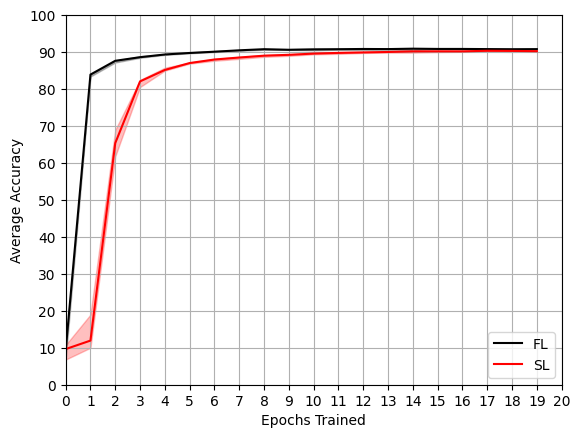
\includegraphics[width=300px]{aeg1}
	\caption{Comparing Accuracy of FL and SL with 6000 Data Samples per Node}
	\label{aeg1}
\end{figure}

\begin{figure}[H]
	\center{\textbf{Accuracy by Training Step for 1000 Samples}} \\
	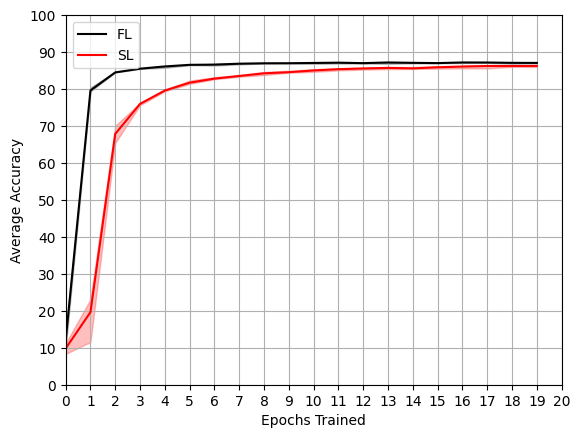
\includegraphics[width=300px]{aeg2}
	\caption{Comparing Accuracy of FL and SL with 1000 Data Samples per Node}
	\label{aeg2}
\end{figure}

\begin{figure}[H]
	\center{\textbf{Accuracy by Training Step for 100 Samples}} \\
	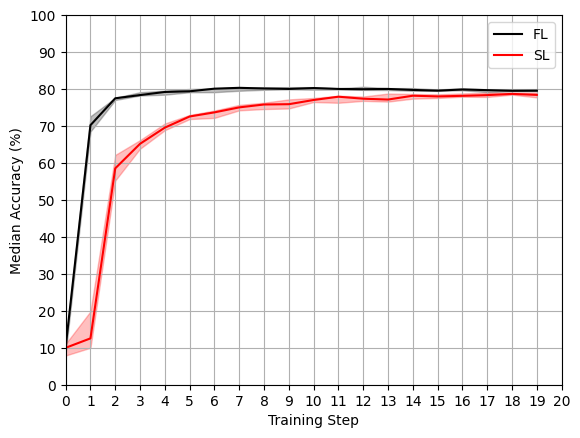
\includegraphics[width=300px]{aeg3}
	\caption{Comparing Accuracy of FL and SL with 100 Data Samples per Node}
	\label{aeg3}
\end{figure}

\subsection{Analysis}

\todo{Write this out}

\begin{itemize}
	\item Clear drop in accuracy when data volume is reduced
	\item SL Consistently performs within a very small margin of FL when looking at peak accuracy
	\item SL is consistently slower to converge than FL
	\item SL has a higher variation in nodes accuracies at the beginning but quickly converges. However, it is much slower to converge on the 100 samples run
	\item Overfitting does not seem to be a problem with either method
\end{itemize}

\section{Dense Network Performance with Node Dropout}

\todo{Do this experiment - it really shouldn't take tong}

the same but this time dropout nodes. Try with and without filtering to show that it increases fault tolerance

To do this, test where a certain number of nodes drop out at step 1, 2, 3, etc

\section{Sparse Network Performance}
In reality, it is uncommon for each node to be linked with every other node. To replicate this scenario, the present study employs a technique to generate a network of nodes with a specific density. It is important to note that, moving forward, density refers to an artificial metric and is not associated with the physical definition of density. When density is set to 0, the network is minimally linked, meaning that each node has at least one indirect path to every other node, but the minimal number of connections required to accomplish this exist. When density is set to 1, all nodes are connected to one another. Since this measure may not provide a straightforward indicator of network density, two additional metrics will be provided:  Mean Minimum Hops (MMH) and Mean Connections per Node (MCPN). MMH denotes the mean number of transitions required to get from a node to another node in the network. MCPN denotes the average nubmer of connections a given node possess.

To ensure good test coverage for a multitude of possible deployment conditions, multiple densities were tested for each count of data. Table \ref{sparsedensities} lists the densities that were tested along with their corresponding MMH and MCPN. To help the reader to visualise the different density levels, Figure \ref{densfig} shows a visual representation of an example network that was generated for each density.

\begin{table}[H]
	\centering
	\begin{tabular}{l|l|l}
		Density & MMH & MCPN \\ \hline
		1 & 1.0 & 9.0 \\
		0.75    & 1.2 & 7.2  \\
		0.5    & 1.4 & 5.4  \\
		0.25    & 1.7 & 3.6  \\
		0    & 3.0 & 1.8  \\
	\end{tabular}
	\caption{The statistics for different density levels} \label{sparsedensities}
\end{table}

\begin{figure}[H]
	\centering
	\begin{subfigure}[b]{0.35\textwidth}
		\centering
		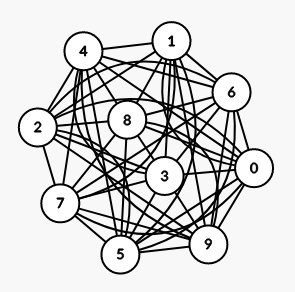
\includegraphics[width=\textwidth]{sparsegraph100}
		\caption{$density=1.0$}
	\end{subfigure}
	\begin{subfigure}[b]{0.35\textwidth}
		\centering
		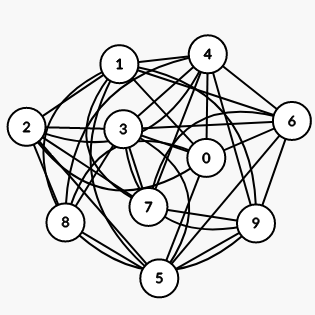
\includegraphics[width=\textwidth]{sparsegraph75}
		\caption{$density=0.75$}
	\end{subfigure}
	\begin{subfigure}[b]{0.35\textwidth}
		\centering
		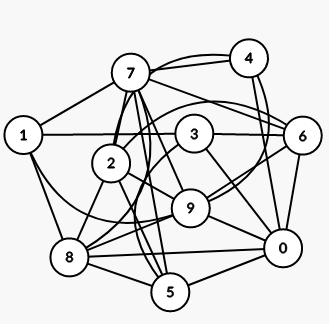
\includegraphics[width=\textwidth]{sparsegraph50}
		\caption{$density=0.5$}
	\end{subfigure}
	\begin{subfigure}[b]{0.35\textwidth}
		\centering
		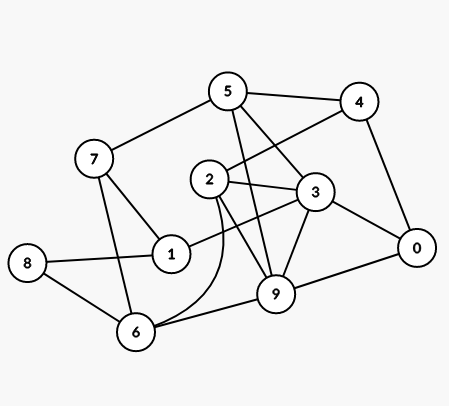
\includegraphics[width=\textwidth]{sparsegraph25}
		\caption{$density=0.25$}
	\end{subfigure}
	\begin{subfigure}[b]{0.35\textwidth}
		\centering
		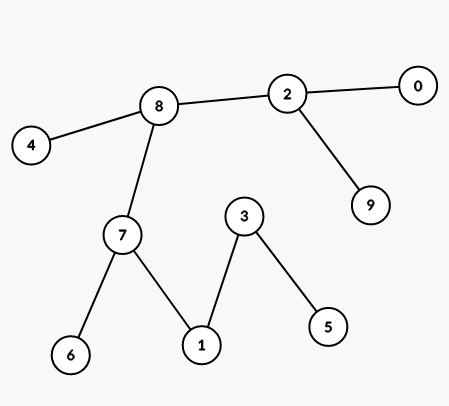
\includegraphics[width=\textwidth]{sparsegraph0}
		\caption{$density=0.0$}
	\end{subfigure}
	\caption{Example networks of nodes generated for each density level, visualised using https://csacademy.com/app/graph\_editor/. \todo{Reference the previous website correctly}}. Each time a simulation is started, a new random network is generated for that simulation.
\end{figure}


In this section, FL is not tested. This is because the only thing FL can do if the server is not directly connected to a node is try to relay the model updates through other nodes or just ignore the disconnected node. For the reasons mentioned in Section \ref{relay}, relaying is not always a good solution, so the decision was made to only test SL in this test.


\subsection{Results}

\todo{Again, maby write somthing here? I'm not sure what to put though.}

\begin{figure}[H] 
	\center{\textbf{Accuracy by Training Step for 6000 Samples for Different Densities}} \\
	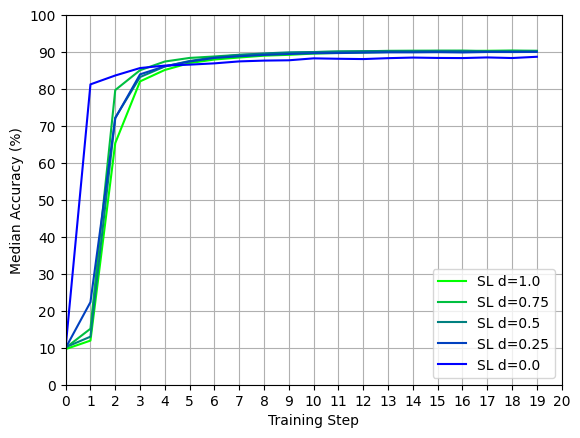
\includegraphics[width=300px]{aeg4}
	\caption{Comparing Accuracy of SL with 6000 Data Samples per Node and varying network density}
	\label{aeg4}
\end{figure}

\begin{figure}[H]
	\center{\textbf{Accuracy by Training Step for 1000 Samples for Different Densities}} \\
	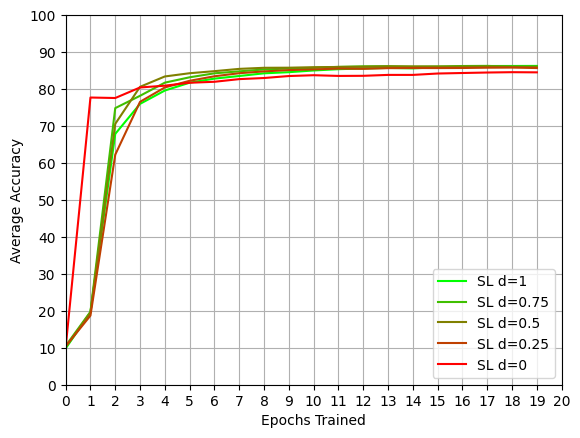
\includegraphics[width=300px]{aeg5}
	\caption{Comparing Accuracy of SL with 1000 Data Samples per Node and varying network density}
	\label{aeg5}
\end{figure}

\begin{figure}[H]
	\center{\textbf{Accuracy by Training Step for 100 Samples for Different Densities}} \\
	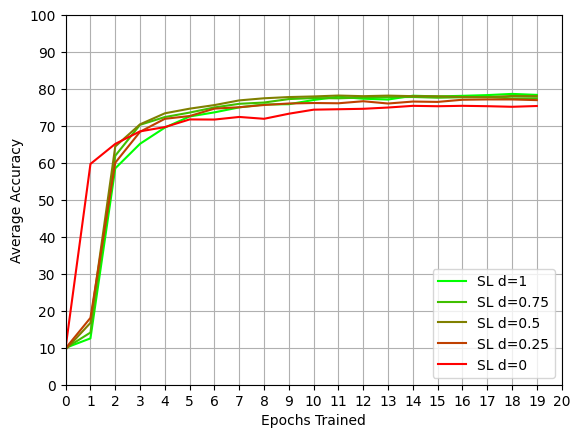
\includegraphics[width=300px]{aeg6}
	\caption{Comparing Accuracy of SL with 100 Data Samples per Node and varying network density}
	\label{aeg6}
\end{figure}

\subsection{Analysis}
\todo{Write this out}

\begin{itemize}
	\item The difference in training performance is negligible until you get the the minimally connected network
	\item The minimally connected network seems to perform better initially but I think this is because the nodes are not fully synced as there is a lot of variation through the network, allowing much faster training. Also note that gamma is much lower for the minimally connected network and this is one of the symptoms of a low gamma.
	\item I don't really know what else to say other than IT WORKS!!!!
\end{itemize}

\section{Sparse Network Performance with Dropout}
\todo{Do this experiment - it really shouldn't take tong}